\begin{center}
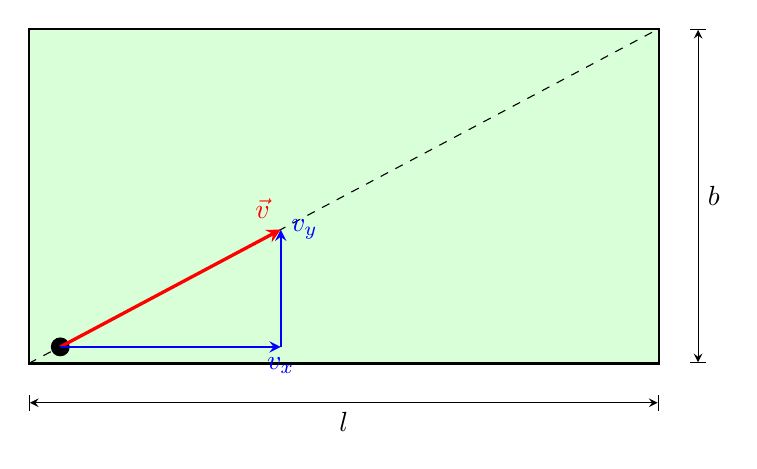
\begin{tikzpicture}[>=stealth]
 \fill[green!15] (0,0) rectangle (8,4.25);
 \draw[thick] (0,0) rectangle (8,4.25);
 \draw[dashed] (0,0) -- (8,4.25);
 \fill (0.4,0.21) circle (0.12);
 \draw[->, very thick, red] (0.4,0.21) -- (3.2,1.70) node[above left] {$\vec v$};
 \draw[->, thick, blue] (0.4,0.21) -- (3.2,0.21) node[below] {$v_x$};
 \draw[->, thick, blue] (3.2,0.21) -- (3.2,1.70) node[right] {$v_y$};
 \draw[|<->|] (0,-0.5) -- (8,-0.5) node[midway, below] {$l$};
 \draw[|<->|] (8.5,0) -- (8.5,4.25) node[midway, right] {$b$};
\end{tikzpicture}
\end{center}

Die Kugel rollt gleichförmig. In der Zeit $t$ legt sie parallel zur Längsseite die Strecke $l$ und parallel zur Breitseite die Strecke $b$ zurück:
\begin{align}
 v_x &= \vxF = \frac{\lTi}{\tBi} = \vx \approx \result{\vxP{0}{2}} \\
 v_y &= \vyF = \frac{\bTi}{\tBi} = \vy \approx \result{\vyP{0}{2}}
\end{align}
Der Betrag des Geschwindigkeitsvektors ist die Länge der Diagonale geteilt durch die Zeit, oder gleichwertig $v = \sqrt{v_x^2+v_y^2}$:
\begin{align}
 v &= \vrF \\
   &= \frac{\sqrt{\left(\lTi\right)^2+\left(\bTi\right)^2}}{\tBi} \\
   &= \vr \approx \result{\vrP{0}{2}}
\end{align}
